\documentclass[1p]{elsarticle_modified}
%\bibliographystyle{elsarticle-num}

%\usepackage[colorlinks]{hyperref}
%\usepackage{abbrmath_seonhwa} %\Abb, \Ascr, \Acal ,\Abf, \Afrak
\usepackage{amsfonts}
\usepackage{amssymb}
\usepackage{amsmath}
\usepackage{amsthm}
\usepackage{scalefnt}
\usepackage{amsbsy}
\usepackage{kotex}
\usepackage{caption}
\usepackage{subfig}
\usepackage{color}
\usepackage{graphicx}
\usepackage{xcolor} %% white, black, red, green, blue, cyan, magenta, yellow
\usepackage{float}
\usepackage{setspace}
\usepackage{hyperref}

\usepackage{tikz}
\usetikzlibrary{arrows}

\usepackage{multirow}
\usepackage{array} % fixed length table
\usepackage{hhline}

%%%%%%%%%%%%%%%%%%%%%
\makeatletter
\renewcommand*\env@matrix[1][\arraystretch]{%
	\edef\arraystretch{#1}%
	\hskip -\arraycolsep
	\let\@ifnextchar\new@ifnextchar
	\array{*\c@MaxMatrixCols c}}
\makeatother %https://tex.stackexchange.com/questions/14071/how-can-i-increase-the-line-spacing-in-a-matrix
%%%%%%%%%%%%%%%

\usepackage[normalem]{ulem}

\newcommand{\msout}[1]{\ifmmode\text{\sout{\ensuremath{#1}}}\else\sout{#1}\fi}
%SOURCE: \msout is \stkout macro in https://tex.stackexchange.com/questions/20609/strikeout-in-math-mode

\newcommand{\cancel}[1]{
	\ifmmode
	{\color{red}\msout{#1}}
	\else
	{\color{red}\sout{#1}}
	\fi
}

\newcommand{\add}[1]{
	{\color{blue}\uwave{#1}}
}

\newcommand{\replace}[2]{
	\ifmmode
	{\color{red}\msout{#1}}{\color{blue}\uwave{#2}}
	\else
	{\color{red}\sout{#1}}{\color{blue}\uwave{#2}}
	\fi
}

\newcommand{\Sol}{\mathcal{S}} %segment
\newcommand{\D}{D} %diagram
\newcommand{\A}{\mathcal{A}} %arc


%%%%%%%%%%%%%%%%%%%%%%%%%%%%%5 test

\def\sl{\operatorname{\textup{SL}}(2,\Cbb)}
\def\psl{\operatorname{\textup{PSL}}(2,\Cbb)}
\def\quan{\mkern 1mu \triangleright \mkern 1mu}

\theoremstyle{definition}
\newtheorem{thm}{Theorem}[section]
\newtheorem{prop}[thm]{Proposition}
\newtheorem{lem}[thm]{Lemma}
\newtheorem{ques}[thm]{Question}
\newtheorem{cor}[thm]{Corollary}
\newtheorem{defn}[thm]{Definition}
\newtheorem{exam}[thm]{Example}
\newtheorem{rmk}[thm]{Remark}
\newtheorem{alg}[thm]{Algorithm}

\newcommand{\I}{\sqrt{-1}}
\begin{document}

%\begin{frontmatter}
%
%\title{Boundary parabolic representations of knots up to 8 crossings}
%
%%% Group authors per affiliation:
%\author{Yunhi Cho} 
%\address{Department of Mathematics, University of Seoul, Seoul, Korea}
%\ead{yhcho@uos.ac.kr}
%
%
%\author{Seonhwa Kim} %\fnref{s_kim}}
%\address{Center for Geometry and Physics, Institute for Basic Science, Pohang, 37673, Korea}
%\ead{ryeona17@ibs.re.kr}
%
%\author{Hyuk Kim}
%\address{Department of Mathematical Sciences, Seoul National University, Seoul 08826, Korea}
%\ead{hyukkim@snu.ac.kr}
%
%\author{Seokbeom Yoon}
%\address{Department of Mathematical Sciences, Seoul National University, Seoul, 08826,  Korea}
%\ead{sbyoon15@snu.ac.kr}
%
%\begin{abstract}
%We find all boundary parabolic representation of knots up to 8 crossings.
%
%\end{abstract}
%\begin{keyword}
%    \MSC[2010] 57M25 
%\end{keyword}
%
%\end{frontmatter}

%\linenumbers
%\tableofcontents
%
\newcommand\colored[1]{\textcolor{white}{\rule[-0.35ex]{0.8em}{1.4ex}}\kern-0.8em\color{red} #1}%
%\newcommand\colored[1]{\textcolor{white}{ #1}\kern-2.17ex	\textcolor{white}{ #1}\kern-1.81ex	\textcolor{white}{ #1}\kern-2.15ex\color{red}#1	}

{\Large $\underline{11a_{109}~(K11a_{109})}$}

\setlength{\tabcolsep}{10pt}
\renewcommand{\arraystretch}{1.6}
\vspace{1cm}\begin{tabular}{m{100pt}>{\centering\arraybackslash}m{274pt}}
\multirow{5}{120pt}{
	\centering
	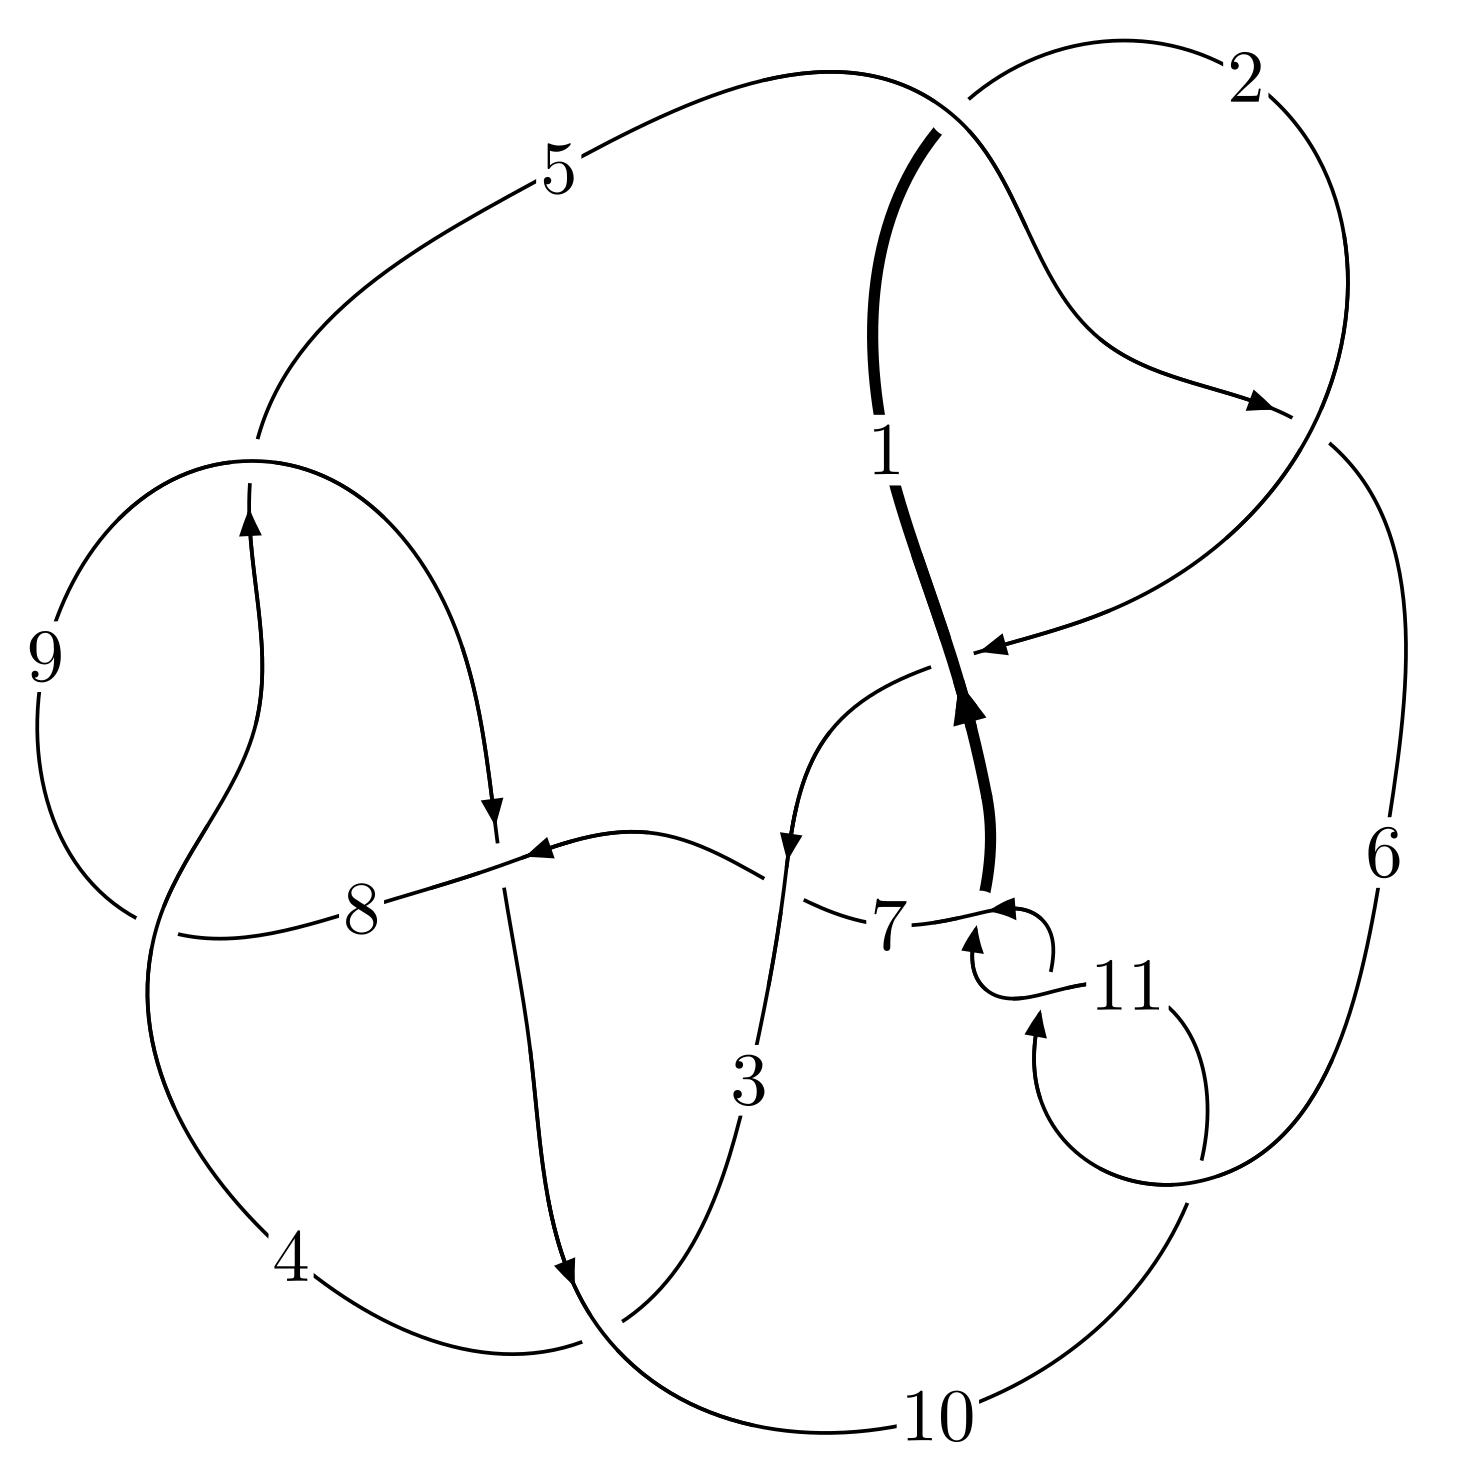
\includegraphics[width=112pt]{../../../GIT/diagram.site/Diagrams/png/358_11a_109.png}\\
\ \ \ A knot diagram\footnotemark}&
\allowdisplaybreaks
\textbf{Linearized knot diagam} \\
\cline{2-2}
 &
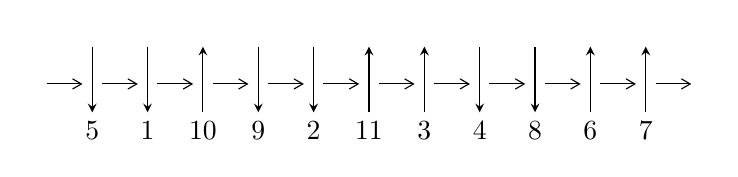
\begin{tikzpicture}[x=20pt, y=17pt]
	% nodes
	\node (C0) at (0, 0) {};
	\node (C1) at (1, 0) {};
	\node (C1U) at (1, +1) {};
	\node (C1D) at (1, -1) {5};

	\node (C2) at (2, 0) {};
	\node (C2U) at (2, +1) {};
	\node (C2D) at (2, -1) {1};

	\node (C3) at (3, 0) {};
	\node (C3U) at (3, +1) {};
	\node (C3D) at (3, -1) {10};

	\node (C4) at (4, 0) {};
	\node (C4U) at (4, +1) {};
	\node (C4D) at (4, -1) {9};

	\node (C5) at (5, 0) {};
	\node (C5U) at (5, +1) {};
	\node (C5D) at (5, -1) {2};

	\node (C6) at (6, 0) {};
	\node (C6U) at (6, +1) {};
	\node (C6D) at (6, -1) {11};

	\node (C7) at (7, 0) {};
	\node (C7U) at (7, +1) {};
	\node (C7D) at (7, -1) {3};

	\node (C8) at (8, 0) {};
	\node (C8U) at (8, +1) {};
	\node (C8D) at (8, -1) {4};

	\node (C9) at (9, 0) {};
	\node (C9U) at (9, +1) {};
	\node (C9D) at (9, -1) {8};

	\node (C10) at (10, 0) {};
	\node (C10U) at (10, +1) {};
	\node (C10D) at (10, -1) {6};

	\node (C11) at (11, 0) {};
	\node (C11U) at (11, +1) {};
	\node (C11D) at (11, -1) {7};
	\node (C12) at (12, 0) {};

	% arrows
	\draw[->,>={angle 60}]
	(C0) edge (C1) (C1) edge (C2) (C2) edge (C3) (C3) edge (C4) (C4) edge (C5) (C5) edge (C6) (C6) edge (C7) (C7) edge (C8) (C8) edge (C9) (C9) edge (C10) (C10) edge (C11) (C11) edge (C12) ;	\draw[->,>=stealth]
	(C1U) edge (C1D) (C2U) edge (C2D) (C3D) edge (C3U) (C4U) edge (C4D) (C5U) edge (C5D) (C6D) edge (C6U) (C7D) edge (C7U) (C8U) edge (C8D) (C9U) edge (C9D) (C10D) edge (C10U) (C11D) edge (C11U) ;
	\end{tikzpicture} \\
\hhline{~~} \\& 
\textbf{Solving Sequence} \\ \cline{2-2} 
 &
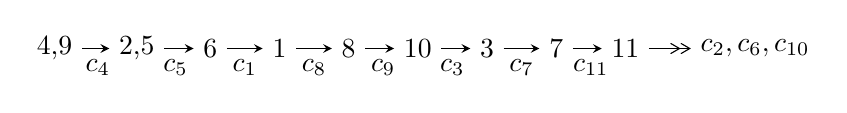
\begin{tikzpicture}[x=25pt, y=7pt]
	% node
	\node (A0) at (-1/8, 0) {4,9};
	\node (A1) at (17/16, 0) {2,5};
	\node (A2) at (17/8, 0) {6};
	\node (A3) at (25/8, 0) {1};
	\node (A4) at (33/8, 0) {8};
	\node (A5) at (41/8, 0) {10};
	\node (A6) at (49/8, 0) {3};
	\node (A7) at (57/8, 0) {7};
	\node (A8) at (65/8, 0) {11};
	\node (C1) at (1/2, -1) {$c_{4}$};
	\node (C2) at (13/8, -1) {$c_{5}$};
	\node (C3) at (21/8, -1) {$c_{1}$};
	\node (C4) at (29/8, -1) {$c_{8}$};
	\node (C5) at (37/8, -1) {$c_{9}$};
	\node (C6) at (45/8, -1) {$c_{3}$};
	\node (C7) at (53/8, -1) {$c_{7}$};
	\node (C8) at (61/8, -1) {$c_{11}$};
	\node (A9) at (10, 0) {$c_{2},c_{6},c_{10}$};

	% edge
	\draw[->,>=stealth]	
	(A0) edge (A1) (A1) edge (A2) (A2) edge (A3) (A3) edge (A4) (A4) edge (A5) (A5) edge (A6) (A6) edge (A7) (A7) edge (A8) ;
	\draw[->>,>={angle 60}]	
	(A8) edge (A9);
\end{tikzpicture} \\ 

\end{tabular} \\

\footnotetext{
The image of knot diagram is generated by the software ``\textbf{Draw programme}" developed by Andrew Bartholomew(\url{http://www.layer8.co.uk/maths/draw/index.htm\#Running-draw}), where we modified some parts for our purpose(\url{https://github.com/CATsTAILs/LinksPainter}).
}\phantom \\ \newline 
\centering \textbf{Ideals for irreducible components\footnotemark of $X_{\text{par}}$} 
 
\begin{align*}
I^u_{1}&=\langle 
u^{45}-11 u^{43}+\cdots+4 b-2 u,\;u^{45}-10 u^{43}+\cdots+4 a-4,\;u^{47}+2 u^{46}+\cdots+4 u+2\rangle \\
I^u_{2}&=\langle 
110 u^5 a^2-28 u^5 a+\cdots-169 a+180,\\
\phantom{I^u_{2}}&\phantom{= \langle  }-2 u^4 a^2- u^5 a+2 u^3 a^2+4 u^4 a+u^5+2 a^2 u^2+2 u^3 a+u^4+a^3-2 a^2 u-5 u^2 a- u^3+4 a u+2 u^2+a-1,\\
\phantom{I^u_{2}}&\phantom{= \langle  }u^6- u^5- u^4+2 u^3- u+1\rangle \\
I^u_{3}&=\langle 
u^3+u^2+b- u+1,\;u^3-2 u^2+2 a+6,\;u^4-2 u^2+2\rangle \\
\\
I^v_{1}&=\langle 
a,\;b+1,\;v-1\rangle \\
\end{align*}
\raggedright * 4 irreducible components of $\dim_{\mathbb{C}}=0$, with total 70 representations.\\
\footnotetext{All coefficients of polynomials are rational numbers. But the coefficients are sometimes approximated in decimal forms when there is not enough margin.}
\newpage
\renewcommand{\arraystretch}{1}
\centering \section*{I. $I^u_{1}= \langle u^{45}-11 u^{43}+\cdots+4 b-2 u,\;u^{45}-10 u^{43}+\cdots+4 a-4,\;u^{47}+2 u^{46}+\cdots+4 u+2 \rangle$}
\flushleft \textbf{(i) Arc colorings}\\
\begin{tabular}{m{7pt} m{180pt} m{7pt} m{180pt} }
\flushright $a_{4}=$&$\begin{pmatrix}1\\0\end{pmatrix}$ \\
\flushright $a_{9}=$&$\begin{pmatrix}0\\u\end{pmatrix}$ \\
\flushright $a_{2}=$&$\begin{pmatrix}-\frac{1}{4} u^{45}+\frac{5}{2} u^{43}+\cdots-\frac{1}{2} u^3+1\\-\frac{1}{4} u^{45}+\frac{11}{4} u^{43}+\cdots+\frac{1}{2} u^2+\frac{1}{2} u\end{pmatrix}$ \\
\flushright $a_{5}=$&$\begin{pmatrix}1\\u^2\end{pmatrix}$ \\
\flushright $a_{6}=$&$\begin{pmatrix}-\frac{1}{2} u^{46}+\frac{11}{2} u^{44}+\cdots-\frac{1}{2} u+\frac{1}{2}\\- u^{46}- u^{45}+\cdots-\frac{7}{2} u-1\end{pmatrix}$ \\
\flushright $a_{1}=$&$\begin{pmatrix}-\frac{1}{2} u^{46}-\frac{3}{4} u^{45}+\cdots-\frac{1}{2} u+\frac{1}{2}\\-\frac{3}{4} u^{45}+\frac{33}{4} u^{43}+\cdots-\frac{1}{2} u-1\end{pmatrix}$ \\
\flushright $a_{8}=$&$\begin{pmatrix}u\\u\end{pmatrix}$ \\
\flushright $a_{10}=$&$\begin{pmatrix}- u^3\\- u^3+u\end{pmatrix}$ \\
\flushright $a_{3}=$&$\begin{pmatrix}u^6- u^4+1\\u^6-2 u^4+u^2\end{pmatrix}$ \\
\flushright $a_{7}=$&$\begin{pmatrix}- u^{11}+2 u^9-2 u^7+u^3\\- u^{11}+3 u^9-4 u^7+3 u^5- u^3+u\end{pmatrix}$ \\
\flushright $a_{11}=$&$\begin{pmatrix}-\frac{1}{4} u^{34}+2 u^{32}+\cdots+\frac{1}{2} u+\frac{1}{2}\\-\frac{1}{4} u^{36}+2 u^{34}+\cdots+\frac{1}{2} u^2+u\end{pmatrix}$\\ \flushright $a_{11}=$&$\begin{pmatrix}-\frac{1}{4} u^{34}+2 u^{32}+\cdots+\frac{1}{2} u+\frac{1}{2}\\-\frac{1}{4} u^{36}+2 u^{34}+\cdots+\frac{1}{2} u^2+u\end{pmatrix}$\\&\end{tabular}
\flushleft \textbf{(ii) Obstruction class $= -1$}\\~\\
\flushleft \textbf{(iii) Cusp Shapes $= -2 u^{46}+22 u^{44}+\cdots-4 u^2+2 u$}\\~\\
\newpage\renewcommand{\arraystretch}{1}
\flushleft \textbf{(iv) u-Polynomials at the component}\newline \\
\begin{tabular}{m{50pt}|m{274pt}}
Crossings & \hspace{64pt}u-Polynomials at each crossing \\
\hline $$\begin{aligned}c_{1},c_{5}\end{aligned}$$&$\begin{aligned}
&u^{47}+2 u^{46}+\cdots-5 u+5
\end{aligned}$\\
\hline $$\begin{aligned}c_{2}\end{aligned}$$&$\begin{aligned}
&u^{47}+18 u^{46}+\cdots+445 u+25
\end{aligned}$\\
\hline $$\begin{aligned}c_{3}\end{aligned}$$&$\begin{aligned}
&u^{47}+6 u^{46}+\cdots+736 u+128
\end{aligned}$\\
\hline $$\begin{aligned}c_{4},c_{8}\end{aligned}$$&$\begin{aligned}
&u^{47}+2 u^{46}+\cdots+4 u+2
\end{aligned}$\\
\hline $$\begin{aligned}c_{6},c_{10},c_{11}\end{aligned}$$&$\begin{aligned}
&u^{47}-2 u^{46}+\cdots+23 u+5
\end{aligned}$\\
\hline $$\begin{aligned}c_{7}\end{aligned}$$&$\begin{aligned}
&u^{47}-2 u^{46}+\cdots-3652 u+3866
\end{aligned}$\\
\hline $$\begin{aligned}c_{9}\end{aligned}$$&$\begin{aligned}
&u^{47}+22 u^{46}+\cdots+8 u+4
\end{aligned}$\\
\hline
\end{tabular}\\~\\
\newpage\renewcommand{\arraystretch}{1}
\flushleft \textbf{(v) Riley Polynomials at the component}\newline \\
\begin{tabular}{m{50pt}|m{274pt}}
Crossings & \hspace{64pt}Riley Polynomials at each crossing \\
\hline $$\begin{aligned}c_{1},c_{5}\end{aligned}$$&$\begin{aligned}
&y^{47}-18 y^{46}+\cdots+445 y-25
\end{aligned}$\\
\hline $$\begin{aligned}c_{2}\end{aligned}$$&$\begin{aligned}
&y^{47}+30 y^{46}+\cdots-49175 y-625
\end{aligned}$\\
\hline $$\begin{aligned}c_{3}\end{aligned}$$&$\begin{aligned}
&y^{47}+10 y^{46}+\cdots-154624 y-16384
\end{aligned}$\\
\hline $$\begin{aligned}c_{4},c_{8}\end{aligned}$$&$\begin{aligned}
&y^{47}-22 y^{46}+\cdots+8 y-4
\end{aligned}$\\
\hline $$\begin{aligned}c_{6},c_{10},c_{11}\end{aligned}$$&$\begin{aligned}
&y^{47}-50 y^{46}+\cdots-211 y-25
\end{aligned}$\\
\hline $$\begin{aligned}c_{7}\end{aligned}$$&$\begin{aligned}
&y^{47}-14 y^{46}+\cdots+245188856 y-14945956
\end{aligned}$\\
\hline $$\begin{aligned}c_{9}\end{aligned}$$&$\begin{aligned}
&y^{47}+6 y^{46}+\cdots-96 y-16
\end{aligned}$\\
\hline
\end{tabular}\\~\\
\newpage\flushleft \textbf{(vi) Complex Volumes and Cusp Shapes}
$$\begin{array}{c|c|c}  
\text{Solutions to }I^u_{1}& \I (\text{vol} + \sqrt{-1}CS) & \text{Cusp shape}\\
 \hline 
\begin{aligned}
u &= \phantom{-}0.637057 + 0.718687 I \\
a &= -0.721070 + 1.203990 I \\
b &= \phantom{-}0.0489452 - 0.0612350 I\end{aligned}
 & \phantom{-}7.88170 - 7.13370 I & \phantom{-}4.69775 + 5.86187 I \\ \hline\begin{aligned}
u &= \phantom{-}0.637057 - 0.718687 I \\
a &= -0.721070 - 1.203990 I \\
b &= \phantom{-}0.0489452 + 0.0612350 I\end{aligned}
 & \phantom{-}7.88170 + 7.13370 I & \phantom{-}4.69775 - 5.86187 I \\ \hline\begin{aligned}
u &= -0.571455 + 0.734273 I \\
a &= \phantom{-}0.246152 + 0.401075 I \\
b &= \phantom{-}0.880555 + 0.625675 I\end{aligned}
 & \phantom{-}9.33252 + 1.08584 I & \phantom{-}6.61100 - 0.78668 I \\ \hline\begin{aligned}
u &= -0.571455 - 0.734273 I \\
a &= \phantom{-}0.246152 - 0.401075 I \\
b &= \phantom{-}0.880555 - 0.625675 I\end{aligned}
 & \phantom{-}9.33252 - 1.08584 I & \phantom{-}6.61100 + 0.78668 I \\ \hline\begin{aligned}
u &= \phantom{-}1.006040 + 0.471862 I \\
a &= \phantom{-}0.029772 - 0.657677 I \\
b &= \phantom{-}0.257242 - 0.932477 I\end{aligned}
 & -0.11745 - 4.26570 I & \phantom{-}1.86221 + 7.53589 I \\ \hline\begin{aligned}
u &= \phantom{-}1.006040 - 0.471862 I \\
a &= \phantom{-}0.029772 + 0.657677 I \\
b &= \phantom{-}0.257242 + 0.932477 I\end{aligned}
 & -0.11745 + 4.26570 I & \phantom{-}1.86221 - 7.53589 I \\ \hline\begin{aligned}
u &= -0.406762 + 0.786472 I \\
a &= \phantom{-}0.118369 - 0.344190 I \\
b &= \phantom{-}0.192922 - 0.870022 I\end{aligned}
 & \phantom{-}8.45114 - 3.90837 I & \phantom{-}6.00297 + 1.23296 I \\ \hline\begin{aligned}
u &= -0.406762 - 0.786472 I \\
a &= \phantom{-}0.118369 + 0.344190 I \\
b &= \phantom{-}0.192922 + 0.870022 I\end{aligned}
 & \phantom{-}8.45114 + 3.90837 I & \phantom{-}6.00297 - 1.23296 I \\ \hline\begin{aligned}
u &= \phantom{-}0.359333 + 0.808292 I \\
a &= -0.860558 - 0.927434 I \\
b &= \phantom{-}2.13804 - 0.70182 I\end{aligned}
 & \phantom{-}6.36842 + 9.89029 I & \phantom{-}3.34606 - 5.56719 I \\ \hline\begin{aligned}
u &= \phantom{-}0.359333 - 0.808292 I \\
a &= -0.860558 + 0.927434 I \\
b &= \phantom{-}2.13804 + 0.70182 I\end{aligned}
 & \phantom{-}6.36842 - 9.89029 I & \phantom{-}3.34606 + 5.56719 I\\
 \hline 
 \end{array}$$\newpage$$\begin{array}{c|c|c}  
\text{Solutions to }I^u_{1}& \I (\text{vol} + \sqrt{-1}CS) & \text{Cusp shape}\\
 \hline 
\begin{aligned}
u &= \phantom{-}1.099960 + 0.219524 I \\
a &= \phantom{-}2.12278 + 0.02040 I \\
b &= \phantom{-}1.40098 + 1.56081 I\end{aligned}
 & -4.03460 + 3.27231 I & -6.93849 - 3.87386 I \\ \hline\begin{aligned}
u &= \phantom{-}1.099960 - 0.219524 I \\
a &= \phantom{-}2.12278 - 0.02040 I \\
b &= \phantom{-}1.40098 - 1.56081 I\end{aligned}
 & -4.03460 - 3.27231 I & -6.93849 + 3.87386 I \\ \hline\begin{aligned}
u &= \phantom{-}1.117490 + 0.132112 I \\
a &= \phantom{-}0.871978 + 0.879966 I \\
b &= \phantom{-}0.365572 + 0.512413 I\end{aligned}
 & \phantom{-}3.39185 + 1.64022 I & \phantom{-}0.179783 - 0.219910 I \\ \hline\begin{aligned}
u &= \phantom{-}1.117490 - 0.132112 I \\
a &= \phantom{-}0.871978 - 0.879966 I \\
b &= \phantom{-}0.365572 - 0.512413 I\end{aligned}
 & \phantom{-}3.39185 - 1.64022 I & \phantom{-}0.179783 + 0.219910 I \\ \hline\begin{aligned}
u &= -0.998163 + 0.550991 I \\
a &= -0.315047 + 0.102429 I \\
b &= -0.898334 - 0.169658 I\end{aligned}
 & \phantom{-}0.241182 + 1.057240 I & \phantom{-}0.289576 + 0.557042 I \\ \hline\begin{aligned}
u &= -0.998163 - 0.550991 I \\
a &= -0.315047 - 0.102429 I \\
b &= -0.898334 + 0.169658 I\end{aligned}
 & \phantom{-}0.241182 - 1.057240 I & \phantom{-}0.289576 - 0.557042 I \\ \hline\begin{aligned}
u &= -0.568933 + 0.644352 I \\
a &= -0.15650 - 1.49843 I \\
b &= -0.187633 - 0.331112 I\end{aligned}
 & \phantom{-}1.50796 + 3.62695 I & \phantom{-}2.13655 - 6.26888 I \\ \hline\begin{aligned}
u &= -0.568933 - 0.644352 I \\
a &= -0.15650 + 1.49843 I \\
b &= -0.187633 + 0.331112 I\end{aligned}
 & \phantom{-}1.50796 - 3.62695 I & \phantom{-}2.13655 + 6.26888 I \\ \hline\begin{aligned}
u &= \phantom{-}0.951297 + 0.631945 I \\
a &= \phantom{-}0.093242 - 0.484467 I \\
b &= -0.390493 + 0.618210 I\end{aligned}
 & \phantom{-}6.94963 + 1.98085 I & \phantom{-}3.48623 - 0.28252 I \\ \hline\begin{aligned}
u &= \phantom{-}0.951297 - 0.631945 I \\
a &= \phantom{-}0.093242 + 0.484467 I \\
b &= -0.390493 - 0.618210 I\end{aligned}
 & \phantom{-}6.94963 - 1.98085 I & \phantom{-}3.48623 + 0.28252 I\\
 \hline 
 \end{array}$$\newpage$$\begin{array}{c|c|c}  
\text{Solutions to }I^u_{1}& \I (\text{vol} + \sqrt{-1}CS) & \text{Cusp shape}\\
 \hline 
\begin{aligned}
u &= \phantom{-}1.108720 + 0.363808 I \\
a &= -2.65417 + 0.58730 I \\
b &= -2.29701 - 1.20468 I\end{aligned}
 & -5.47077 - 3.68113 I & -9.62046 + 4.56447 I \\ \hline\begin{aligned}
u &= \phantom{-}1.108720 - 0.363808 I \\
a &= -2.65417 - 0.58730 I \\
b &= -2.29701 + 1.20468 I\end{aligned}
 & -5.47077 + 3.68113 I & -9.62046 - 4.56447 I \\ \hline\begin{aligned}
u &= -0.365235 + 0.745543 I \\
a &= -0.561966 + 1.294290 I \\
b &= \phantom{-}1.96786 + 0.35399 I\end{aligned}
 & \phantom{-}0.49152 - 5.74739 I & \phantom{-}0.29552 + 5.57964 I \\ \hline\begin{aligned}
u &= -0.365235 - 0.745543 I \\
a &= -0.561966 - 1.294290 I \\
b &= \phantom{-}1.96786 - 0.35399 I\end{aligned}
 & \phantom{-}0.49152 + 5.74739 I & \phantom{-}0.29552 - 5.57964 I \\ \hline\begin{aligned}
u &= -1.165410 + 0.187983 I \\
a &= \phantom{-}2.28007 + 0.42466 I \\
b &= \phantom{-}2.08406 - 1.07708 I\end{aligned}
 & \phantom{-}1.38638 - 7.13549 I & -2.46560 + 4.47635 I \\ \hline\begin{aligned}
u &= -1.165410 - 0.187983 I \\
a &= \phantom{-}2.28007 - 0.42466 I \\
b &= \phantom{-}2.08406 + 1.07708 I\end{aligned}
 & \phantom{-}1.38638 + 7.13549 I & -2.46560 - 4.47635 I \\ \hline\begin{aligned}
u &= -1.005960 + 0.623496 I \\
a &= \phantom{-}1.24908 + 0.75581 I \\
b &= \phantom{-}1.063390 - 0.194010 I\end{aligned}
 & \phantom{-}8.04432 + 4.08182 I & \phantom{-}4.48123 - 4.68553 I \\ \hline\begin{aligned}
u &= -1.005960 - 0.623496 I \\
a &= \phantom{-}1.24908 - 0.75581 I \\
b &= \phantom{-}1.063390 + 0.194010 I\end{aligned}
 & \phantom{-}8.04432 - 4.08182 I & \phantom{-}4.48123 + 4.68553 I \\ \hline\begin{aligned}
u &= -1.111110 + 0.494738 I \\
a &= -1.83321 - 1.25072 I \\
b &= -2.10148 + 0.95562 I\end{aligned}
 & -4.58829 + 3.84650 I & -8.76666 - 3.56046 I \\ \hline\begin{aligned}
u &= -1.111110 - 0.494738 I \\
a &= -1.83321 + 1.25072 I \\
b &= -2.10148 - 0.95562 I\end{aligned}
 & -4.58829 - 3.84650 I & -8.76666 + 3.56046 I\\
 \hline 
 \end{array}$$\newpage$$\begin{array}{c|c|c}  
\text{Solutions to }I^u_{1}& \I (\text{vol} + \sqrt{-1}CS) & \text{Cusp shape}\\
 \hline 
\begin{aligned}
u &= -1.176480 + 0.396630 I \\
a &= -2.40697 - 0.03813 I \\
b &= -2.05844 + 1.68830 I\end{aligned}
 & -1.23516 + 6.21145 I & -1.74487 - 7.02826 I \\ \hline\begin{aligned}
u &= -1.176480 - 0.396630 I \\
a &= -2.40697 + 0.03813 I \\
b &= -2.05844 - 1.68830 I\end{aligned}
 & -1.23516 - 6.21145 I & -1.74487 + 7.02826 I \\ \hline\begin{aligned}
u &= \phantom{-}0.066156 + 0.753461 I \\
a &= \phantom{-}0.967191 + 0.143999 I \\
b &= -1.41080 - 0.53958 I\end{aligned}
 & \phantom{-}2.42833 - 2.22486 I & \phantom{-}2.96572 + 3.27842 I \\ \hline\begin{aligned}
u &= \phantom{-}0.066156 - 0.753461 I \\
a &= \phantom{-}0.967191 - 0.143999 I \\
b &= -1.41080 + 0.53958 I\end{aligned}
 & \phantom{-}2.42833 + 2.22486 I & \phantom{-}2.96572 - 3.27842 I \\ \hline\begin{aligned}
u &= -1.111590 + 0.573138 I \\
a &= \phantom{-}2.03891 + 1.83979 I \\
b &= \phantom{-}3.12984 - 0.32101 I\end{aligned}
 & -1.69804 + 10.75150 I & -2.97142 - 9.27459 I \\ \hline\begin{aligned}
u &= -1.111590 - 0.573138 I \\
a &= \phantom{-}2.03891 - 1.83979 I \\
b &= \phantom{-}3.12984 + 0.32101 I\end{aligned}
 & -1.69804 - 10.75150 I & -2.97142 + 9.27459 I \\ \hline\begin{aligned}
u &= \phantom{-}1.168440 + 0.464509 I \\
a &= -1.31459 + 1.24173 I \\
b &= -2.05354 - 0.47643 I\end{aligned}
 & -0.77532 - 2.18171 I & \phantom{-0.000000 } 0 \\ \hline\begin{aligned}
u &= \phantom{-}1.168440 - 0.464509 I \\
a &= -1.31459 - 1.24173 I \\
b &= -2.05354 + 0.47643 I\end{aligned}
 & -0.77532 + 2.18171 I & \phantom{-0.000000 } 0 \\ \hline\begin{aligned}
u &= -1.108280 + 0.598698 I \\
a &= -0.816787 + 0.770371 I \\
b &= -0.110572 + 0.781750 I\end{aligned}
 & \phantom{-}6.36874 + 9.11603 I & \phantom{-}3.03425 - 5.54417 I \\ \hline\begin{aligned}
u &= -1.108280 - 0.598698 I \\
a &= -0.816787 - 0.770371 I \\
b &= -0.110572 - 0.781750 I\end{aligned}
 & \phantom{-}6.36874 - 9.11603 I & \phantom{-}3.03425 + 5.54417 I\\
 \hline 
 \end{array}$$\newpage$$\begin{array}{c|c|c}  
\text{Solutions to }I^u_{1}& \I (\text{vol} + \sqrt{-1}CS) & \text{Cusp shape}\\
 \hline 
\begin{aligned}
u &= \phantom{-}1.132790 + 0.591464 I \\
a &= \phantom{-}2.36607 - 1.55769 I \\
b &= \phantom{-}3.12191 + 1.03804 I\end{aligned}
 & \phantom{-}4.0697 - 15.1191 I & \phantom{-0.000000 -}0. + 9.40367 I \\ \hline\begin{aligned}
u &= \phantom{-}1.132790 - 0.591464 I \\
a &= \phantom{-}2.36607 + 1.55769 I \\
b &= \phantom{-}3.12191 - 1.03804 I\end{aligned}
 & \phantom{-}4.0697 + 15.1191 I & \phantom{-0.000000 } 0. - 9.40367 I \\ \hline\begin{aligned}
u &= -0.664931\phantom{ +0.000000I} \\
a &= \phantom{-}1.02381\phantom{ +0.000000I} \\
b &= -0.379109\phantom{ +0.000000I}\end{aligned}
 & -1.34703\phantom{ +0.000000I} & -7.25790\phantom{ +0.000000I} \\ \hline\begin{aligned}
u &= \phantom{-}0.448712 + 0.454594 I \\
a &= \phantom{-}1.225200 - 0.260236 I \\
b &= \phantom{-}0.412150 + 0.326959 I\end{aligned}
 & \phantom{-}1.43130 + 0.33753 I & \phantom{-}6.95713 - 1.01845 I \\ \hline\begin{aligned}
u &= \phantom{-}0.448712 - 0.454594 I \\
a &= \phantom{-}1.225200 + 0.260236 I \\
b &= \phantom{-}0.412150 - 0.326959 I\end{aligned}
 & \phantom{-}1.43130 - 0.33753 I & \phantom{-}6.95713 + 1.01845 I \\ \hline\begin{aligned}
u &= -0.174154 + 0.607070 I \\
a &= \phantom{-}1.020160 - 0.035294 I \\
b &= -1.365630 + 0.008684 I\end{aligned}
 & -2.04844 + 0.43724 I & -5.38341 - 0.85631 I \\ \hline\begin{aligned}
u &= -0.174154 - 0.607070 I \\
a &= \phantom{-}1.020160 + 0.035294 I \\
b &= -1.365630 - 0.008684 I\end{aligned}
 & -2.04844 - 0.43724 I & -5.38341 + 0.85631 I\\
 \hline 
 \end{array}$$\newpage\newpage\renewcommand{\arraystretch}{1}
\centering \section*{II. $I^u_{2}= \langle 110 u^5 a^2-28 u^5 a+\cdots-169 a+180,\;- u^5 a+u^5+\cdots+a-1,\;u^6- u^5- u^4+2 u^3- u+1 \rangle$}
\flushleft \textbf{(i) Arc colorings}\\
\begin{tabular}{m{7pt} m{180pt} m{7pt} m{180pt} }
\flushright $a_{4}=$&$\begin{pmatrix}1\\0\end{pmatrix}$ \\
\flushright $a_{9}=$&$\begin{pmatrix}0\\u\end{pmatrix}$ \\
\flushright $a_{2}=$&$\begin{pmatrix}a\\-0.607735 a^{2} u^{5}+0.154696 a u^{5}+\cdots+0.933702 a-0.994475\end{pmatrix}$ \\
\flushright $a_{5}=$&$\begin{pmatrix}1\\u^2\end{pmatrix}$ \\
\flushright $a_{6}=$&$\begin{pmatrix}-0.232044 a^{2} u^{5}-0.359116 a u^{5}+\cdots+1.01105 a+0.165746\\-0.243094 a^{2} u^{5}+0.861878 a u^{5}+\cdots-1.22652 a+1.60221\end{pmatrix}$ \\
\flushright $a_{1}=$&$\begin{pmatrix}-0.607735 a^{2} u^{5}+0.154696 a u^{5}+\cdots+1.93370 a-0.994475\\-1.02762 a^{2} u^{5}+0.552486 a u^{5}+\cdots-0.0939227 a-0.408840\end{pmatrix}$ \\
\flushright $a_{8}=$&$\begin{pmatrix}u\\u\end{pmatrix}$ \\
\flushright $a_{10}=$&$\begin{pmatrix}- u^3\\- u^3+u\end{pmatrix}$ \\
\flushright $a_{3}=$&$\begin{pmatrix}u^5-2 u^3+u\\u^5- u^4-2 u^3+u^2+u-1\end{pmatrix}$ \\
\flushright $a_{7}=$&$\begin{pmatrix}-1\\- u^2\end{pmatrix}$ \\
\flushright $a_{11}=$&$\begin{pmatrix}a\\-0.607735 a^{2} u^{5}+0.154696 a u^{5}+\cdots+0.933702 a-0.994475\end{pmatrix}$\\ \flushright $a_{11}=$&$\begin{pmatrix}a\\-0.607735 a^{2} u^{5}+0.154696 a u^{5}+\cdots+0.933702 a-0.994475\end{pmatrix}$\\&\end{tabular}
\flushleft \textbf{(ii) Obstruction class $= -1$}\\~\\
\flushleft \textbf{(iii) Cusp Shapes $= 4 u^4-4 u^2+4 u+2$}\\~\\
\newpage\renewcommand{\arraystretch}{1}
\flushleft \textbf{(iv) u-Polynomials at the component}\newline \\
\begin{tabular}{m{50pt}|m{274pt}}
Crossings & \hspace{64pt}u-Polynomials at each crossing \\
\hline $$\begin{aligned}c_{1},c_{5},c_{6}\\c_{10},c_{11}\end{aligned}$$&$\begin{aligned}
&u^{18}-6 u^{16}+\cdots+u+1
\end{aligned}$\\
\hline $$\begin{aligned}c_{2}\end{aligned}$$&$\begin{aligned}
&u^{18}+12 u^{17}+\cdots+u+1
\end{aligned}$\\
\hline $$\begin{aligned}c_{3}\end{aligned}$$&$\begin{aligned}
&(u^6-3 u^5+5 u^4-4 u^3+2 u^2- u+1)^3
\end{aligned}$\\
\hline $$\begin{aligned}c_{4},c_{8}\end{aligned}$$&$\begin{aligned}
&(u^6- u^5- u^4+2 u^3- u+1)^3
\end{aligned}$\\
\hline $$\begin{aligned}c_{7}\end{aligned}$$&$\begin{aligned}
&(u^6+u^5- u^4-2 u^3+u+1)^3
\end{aligned}$\\
\hline $$\begin{aligned}c_{9}\end{aligned}$$&$\begin{aligned}
&(u^6+3 u^5+5 u^4+4 u^3+2 u^2+u+1)^3
\end{aligned}$\\
\hline
\end{tabular}\\~\\
\newpage\renewcommand{\arraystretch}{1}
\flushleft \textbf{(v) Riley Polynomials at the component}\newline \\
\begin{tabular}{m{50pt}|m{274pt}}
Crossings & \hspace{64pt}Riley Polynomials at each crossing \\
\hline $$\begin{aligned}c_{1},c_{5},c_{6}\\c_{10},c_{11}\end{aligned}$$&$\begin{aligned}
&y^{18}-12 y^{17}+\cdots- y+1
\end{aligned}$\\
\hline $$\begin{aligned}c_{2}\end{aligned}$$&$\begin{aligned}
&y^{18}-12 y^{17}+\cdots+7 y+1
\end{aligned}$\\
\hline $$\begin{aligned}c_{3},c_{9}\end{aligned}$$&$\begin{aligned}
&(y^6+y^5+5 y^4+6 y^2+3 y+1)^3
\end{aligned}$\\
\hline $$\begin{aligned}c_{4},c_{7},c_{8}\end{aligned}$$&$\begin{aligned}
&(y^6-3 y^5+5 y^4-4 y^3+2 y^2- y+1)^3
\end{aligned}$\\
\hline
\end{tabular}\\~\\
\newpage\flushleft \textbf{(vi) Complex Volumes and Cusp Shapes}
$$\begin{array}{c|c|c}  
\text{Solutions to }I^u_{2}& \I (\text{vol} + \sqrt{-1}CS) & \text{Cusp shape}\\
 \hline 
\begin{aligned}
u &= -1.002190 + 0.295542 I \\
a &= \phantom{-}0.348652 - 0.303516 I \\
b &= -0.0836886 + 0.0822976 I\end{aligned}
 & -1.89061 + 0.92430 I & -3.71672 - 0.79423 I \\ \hline\begin{aligned}
u &= -1.002190 + 0.295542 I \\
a &= \phantom{-}1.54157 - 0.67011 I \\
b &= \phantom{-}0.02798 - 1.89773 I\end{aligned}
 & -1.89061 + 0.92430 I & -3.71672 - 0.79423 I \\ \hline\begin{aligned}
u &= -1.002190 + 0.295542 I \\
a &= -3.26061 - 1.15289 I \\
b &= -2.46071 + 0.67711 I\end{aligned}
 & -1.89061 + 0.92430 I & -3.71672 - 0.79423 I \\ \hline\begin{aligned}
u &= -1.002190 - 0.295542 I \\
a &= \phantom{-}0.348652 + 0.303516 I \\
b &= -0.0836886 - 0.0822976 I\end{aligned}
 & -1.89061 - 0.92430 I & -3.71672 + 0.79423 I \\ \hline\begin{aligned}
u &= -1.002190 - 0.295542 I \\
a &= \phantom{-}1.54157 + 0.67011 I \\
b &= \phantom{-}0.02798 + 1.89773 I\end{aligned}
 & -1.89061 - 0.92430 I & -3.71672 + 0.79423 I \\ \hline\begin{aligned}
u &= -1.002190 - 0.295542 I \\
a &= -3.26061 + 1.15289 I \\
b &= -2.46071 - 0.67711 I\end{aligned}
 & -1.89061 - 0.92430 I & -3.71672 + 0.79423 I \\ \hline\begin{aligned}
u &= \phantom{-}0.428243 + 0.664531 I \\
a &= \phantom{-}0.466201 + 0.792945 I \\
b &= -0.025081 + 0.674941 I\end{aligned}
 & \phantom{-}1.89061 + 0.92430 I & \phantom{-}3.71672 - 0.79423 I \\ \hline\begin{aligned}
u &= \phantom{-}0.428243 + 0.664531 I \\
a &= \phantom{-}1.083770 - 0.074988 I \\
b &= -1.56679 + 0.56745 I\end{aligned}
 & \phantom{-}1.89061 + 0.92430 I & \phantom{-}3.71672 - 0.79423 I \\ \hline\begin{aligned}
u &= \phantom{-}0.428243 + 0.664531 I \\
a &= \phantom{-}0.285996 - 1.259370 I \\
b &= \phantom{-}1.42596 - 0.05764 I\end{aligned}
 & \phantom{-}1.89061 + 0.92430 I & \phantom{-}3.71672 - 0.79423 I \\ \hline\begin{aligned}
u &= \phantom{-}0.428243 - 0.664531 I \\
a &= \phantom{-}0.466201 - 0.792945 I \\
b &= -0.025081 - 0.674941 I\end{aligned}
 & \phantom{-}1.89061 - 0.92430 I & \phantom{-}3.71672 + 0.79423 I\\
 \hline 
 \end{array}$$\newpage$$\begin{array}{c|c|c}  
\text{Solutions to }I^u_{2}& \I (\text{vol} + \sqrt{-1}CS) & \text{Cusp shape}\\
 \hline 
\begin{aligned}
u &= \phantom{-}0.428243 - 0.664531 I \\
a &= \phantom{-}1.083770 + 0.074988 I \\
b &= -1.56679 - 0.56745 I\end{aligned}
 & \phantom{-}1.89061 - 0.92430 I & \phantom{-}3.71672 + 0.79423 I \\ \hline\begin{aligned}
u &= \phantom{-}0.428243 - 0.664531 I \\
a &= \phantom{-}0.285996 + 1.259370 I \\
b &= \phantom{-}1.42596 + 0.05764 I\end{aligned}
 & \phantom{-}1.89061 - 0.92430 I & \phantom{-}3.71672 + 0.79423 I \\ \hline\begin{aligned}
u &= \phantom{-}1.073950 + 0.558752 I \\
a &= -0.789928 - 0.420050 I \\
b &= -0.640192 - 0.601752 I\end{aligned}
 & \phantom{-0.000000 } -5.69302 I & \phantom{-0.000000 -}0. + 5.51057 I \\ \hline\begin{aligned}
u &= \phantom{-}1.073950 + 0.558752 I \\
a &= \phantom{-}1.29540 - 1.82419 I \\
b &= \phantom{-}2.40293 - 0.55520 I\end{aligned}
 & \phantom{-0.000000 } -5.69302 I & \phantom{-0.000000 -}0. + 5.51057 I \\ \hline\begin{aligned}
u &= \phantom{-}1.073950 + 0.558752 I \\
a &= -1.97105 + 1.48173 I \\
b &= -2.08041 - 1.24333 I\end{aligned}
 & \phantom{-0.000000 } -5.69302 I & \phantom{-0.000000 -}0. + 5.51057 I \\ \hline\begin{aligned}
u &= \phantom{-}1.073950 - 0.558752 I \\
a &= -0.789928 + 0.420050 I \\
b &= -0.640192 + 0.601752 I\end{aligned}
 & \phantom{-0.000000 -}5.69302 I & \phantom{-0.000000 } 0. - 5.51057 I \\ \hline\begin{aligned}
u &= \phantom{-}1.073950 - 0.558752 I \\
a &= \phantom{-}1.29540 + 1.82419 I \\
b &= \phantom{-}2.40293 + 0.55520 I\end{aligned}
 & \phantom{-0.000000 -}5.69302 I & \phantom{-0.000000 } 0. - 5.51057 I \\ \hline\begin{aligned}
u &= \phantom{-}1.073950 - 0.558752 I \\
a &= -1.97105 - 1.48173 I \\
b &= -2.08041 + 1.24333 I\end{aligned}
 & \phantom{-0.000000 -}5.69302 I & \phantom{-0.000000 } 0. - 5.51057 I\\
 \hline 
 \end{array}$$\newpage\newpage\renewcommand{\arraystretch}{1}
\centering \section*{III. $I^u_{3}= \langle u^3+u^2+b- u+1,\;u^3-2 u^2+2 a+6,\;u^4-2 u^2+2 \rangle$}
\flushleft \textbf{(i) Arc colorings}\\
\begin{tabular}{m{7pt} m{180pt} m{7pt} m{180pt} }
\flushright $a_{4}=$&$\begin{pmatrix}1\\0\end{pmatrix}$ \\
\flushright $a_{9}=$&$\begin{pmatrix}0\\u\end{pmatrix}$ \\
\flushright $a_{2}=$&$\begin{pmatrix}-\frac{1}{2} u^3+u^2-3\\- u^3- u^2+u-1\end{pmatrix}$ \\
\flushright $a_{5}=$&$\begin{pmatrix}1\\u^2\end{pmatrix}$ \\
\flushright $a_{6}=$&$\begin{pmatrix}-\frac{1}{2} u^3+u^2-2\\- u^3+u-1\end{pmatrix}$ \\
\flushright $a_{1}=$&$\begin{pmatrix}-\frac{1}{2} u^3+u^2-2\\- u^3+u-1\end{pmatrix}$ \\
\flushright $a_{8}=$&$\begin{pmatrix}u\\u\end{pmatrix}$ \\
\flushright $a_{10}=$&$\begin{pmatrix}- u^3\\- u^3+u\end{pmatrix}$ \\
\flushright $a_{3}=$&$\begin{pmatrix}-1\\- u^2\end{pmatrix}$ \\
\flushright $a_{7}=$&$\begin{pmatrix}u^3\\u^3- u\end{pmatrix}$ \\
\flushright $a_{11}=$&$\begin{pmatrix}-\frac{3}{2} u^3+u^2-2\\-2 u^3+2 u-1\end{pmatrix}$\\ \flushright $a_{11}=$&$\begin{pmatrix}-\frac{3}{2} u^3+u^2-2\\-2 u^3+2 u-1\end{pmatrix}$\\&\end{tabular}
\flushleft \textbf{(ii) Obstruction class $= 1$}\\~\\
\flushleft \textbf{(iii) Cusp Shapes $= 4 u^2-8$}\\~\\
\newpage\renewcommand{\arraystretch}{1}
\flushleft \textbf{(iv) u-Polynomials at the component}\newline \\
\begin{tabular}{m{50pt}|m{274pt}}
Crossings & \hspace{64pt}u-Polynomials at each crossing \\
\hline $$\begin{aligned}c_{1},c_{2},c_{10}\\c_{11}\end{aligned}$$&$\begin{aligned}
&(u+1)^4
\end{aligned}$\\
\hline $$\begin{aligned}c_{3},c_{7}\end{aligned}$$&$\begin{aligned}
&u^4+2 u^2+2
\end{aligned}$\\
\hline $$\begin{aligned}c_{4},c_{8}\end{aligned}$$&$\begin{aligned}
&u^4-2 u^2+2
\end{aligned}$\\
\hline $$\begin{aligned}c_{5},c_{6}\end{aligned}$$&$\begin{aligned}
&(u-1)^4
\end{aligned}$\\
\hline $$\begin{aligned}c_{9}\end{aligned}$$&$\begin{aligned}
&(u^2+2 u+2)^2
\end{aligned}$\\
\hline
\end{tabular}\\~\\
\newpage\renewcommand{\arraystretch}{1}
\flushleft \textbf{(v) Riley Polynomials at the component}\newline \\
\begin{tabular}{m{50pt}|m{274pt}}
Crossings & \hspace{64pt}Riley Polynomials at each crossing \\
\hline $$\begin{aligned}c_{1},c_{2},c_{5}\\c_{6},c_{10},c_{11}\end{aligned}$$&$\begin{aligned}
&(y-1)^4
\end{aligned}$\\
\hline $$\begin{aligned}c_{3},c_{7}\end{aligned}$$&$\begin{aligned}
&(y^2+2 y+2)^2
\end{aligned}$\\
\hline $$\begin{aligned}c_{4},c_{8}\end{aligned}$$&$\begin{aligned}
&(y^2-2 y+2)^2
\end{aligned}$\\
\hline $$\begin{aligned}c_{9}\end{aligned}$$&$\begin{aligned}
&(y^2+4)^2
\end{aligned}$\\
\hline
\end{tabular}\\~\\
\newpage\flushleft \textbf{(vi) Complex Volumes and Cusp Shapes}
$$\begin{array}{c|c|c}  
\text{Solutions to }I^u_{3}& \I (\text{vol} + \sqrt{-1}CS) & \text{Cusp shape}\\
 \hline 
\begin{aligned}
u &= \phantom{-}1.098680 + 0.455090 I \\
a &= -2.32180 + 0.22311 I \\
b &= -1.54491 - 2.09868 I\end{aligned}
 & -2.46740 - 3.66386 I & -4.00000 + 4.00000 I \\ \hline\begin{aligned}
u &= \phantom{-}1.098680 - 0.455090 I \\
a &= -2.32180 - 0.22311 I \\
b &= -1.54491 + 2.09868 I\end{aligned}
 & -2.46740 + 3.66386 I & -4.00000 - 4.00000 I \\ \hline\begin{aligned}
u &= -1.098680 + 0.455090 I \\
a &= -1.67820 - 1.77689 I \\
b &= -2.45509 - 0.09868 I\end{aligned}
 & -2.46740 + 3.66386 I & -4.00000 - 4.00000 I \\ \hline\begin{aligned}
u &= -1.098680 - 0.455090 I \\
a &= -1.67820 + 1.77689 I \\
b &= -2.45509 + 0.09868 I\end{aligned}
 & -2.46740 - 3.66386 I & -4.00000 + 4.00000 I\\
 \hline 
 \end{array}$$\newpage\newpage\renewcommand{\arraystretch}{1}
\centering \section*{IV. $I^v_{1}= \langle a,\;b+1,\;v-1 \rangle$}
\flushleft \textbf{(i) Arc colorings}\\
\begin{tabular}{m{7pt} m{180pt} m{7pt} m{180pt} }
\flushright $a_{4}=$&$\begin{pmatrix}1\\0\end{pmatrix}$ \\
\flushright $a_{9}=$&$\begin{pmatrix}1\\0\end{pmatrix}$ \\
\flushright $a_{2}=$&$\begin{pmatrix}0\\-1\end{pmatrix}$ \\
\flushright $a_{5}=$&$\begin{pmatrix}1\\0\end{pmatrix}$ \\
\flushright $a_{6}=$&$\begin{pmatrix}1\\1\end{pmatrix}$ \\
\flushright $a_{1}=$&$\begin{pmatrix}-1\\-1\end{pmatrix}$ \\
\flushright $a_{8}=$&$\begin{pmatrix}1\\0\end{pmatrix}$ \\
\flushright $a_{10}=$&$\begin{pmatrix}1\\0\end{pmatrix}$ \\
\flushright $a_{3}=$&$\begin{pmatrix}1\\0\end{pmatrix}$ \\
\flushright $a_{7}=$&$\begin{pmatrix}1\\0\end{pmatrix}$ \\
\flushright $a_{11}=$&$\begin{pmatrix}0\\-1\end{pmatrix}$\\ \flushright $a_{11}=$&$\begin{pmatrix}0\\-1\end{pmatrix}$\\&\end{tabular}
\flushleft \textbf{(ii) Obstruction class $= 1$}\\~\\
\flushleft \textbf{(iii) Cusp Shapes $= 0$}\\~\\
\newpage\renewcommand{\arraystretch}{1}
\flushleft \textbf{(iv) u-Polynomials at the component}\newline \\
\begin{tabular}{m{50pt}|m{274pt}}
Crossings & \hspace{64pt}u-Polynomials at each crossing \\
\hline $$\begin{aligned}c_{1},c_{10},c_{11}\end{aligned}$$&$\begin{aligned}
&u-1
\end{aligned}$\\
\hline $$\begin{aligned}c_{2},c_{5},c_{6}\end{aligned}$$&$\begin{aligned}
&u+1
\end{aligned}$\\
\hline $$\begin{aligned}c_{3},c_{4},c_{7}\\c_{8},c_{9}\end{aligned}$$&$\begin{aligned}
&u
\end{aligned}$\\
\hline
\end{tabular}\\~\\
\newpage\renewcommand{\arraystretch}{1}
\flushleft \textbf{(v) Riley Polynomials at the component}\newline \\
\begin{tabular}{m{50pt}|m{274pt}}
Crossings & \hspace{64pt}Riley Polynomials at each crossing \\
\hline $$\begin{aligned}c_{1},c_{2},c_{5}\\c_{6},c_{10},c_{11}\end{aligned}$$&$\begin{aligned}
&y-1
\end{aligned}$\\
\hline $$\begin{aligned}c_{3},c_{4},c_{7}\\c_{8},c_{9}\end{aligned}$$&$\begin{aligned}
&y
\end{aligned}$\\
\hline
\end{tabular}\\~\\
\newpage\flushleft \textbf{(vi) Complex Volumes and Cusp Shapes}
$$\begin{array}{c|c|c}  
\text{Solutions to }I^v_{1}& \I (\text{vol} + \sqrt{-1}CS) & \text{Cusp shape}\\
 \hline 
\begin{aligned}
v &= \phantom{-}1.00000\phantom{ +0.000000I} \\
a &= \phantom{-0.000000 } 0 \\
b &= -1.00000\phantom{ +0.000000I}\end{aligned}
 & \phantom{-0.000000 } 0 & \phantom{-0.000000 } 0\\
 \hline 
 \end{array}$$\newpage
\newpage\renewcommand{\arraystretch}{1}
\centering \section*{ V. u-Polynomials}
\begin{tabular}{m{50pt}|m{274pt}}
Crossings & \hspace{64pt}u-Polynomials at each crossing \\
\hline $$\begin{aligned}c_{1}\end{aligned}$$&$\begin{aligned}
&(u-1)(u+1)^4(u^{18}-6 u^{16}+\cdots+u+1)(u^{47}+2 u^{46}+\cdots-5 u+5)
\end{aligned}$\\
\hline $$\begin{aligned}c_{2}\end{aligned}$$&$\begin{aligned}
&((u+1)^5)(u^{18}+12 u^{17}+\cdots+u+1)(u^{47}+18 u^{46}+\cdots+445 u+25)
\end{aligned}$\\
\hline $$\begin{aligned}c_{3}\end{aligned}$$&$\begin{aligned}
&u(u^4+2 u^2+2)(u^6-3 u^5+5 u^4-4 u^3+2 u^2- u+1)^3\\
&\cdot(u^{47}+6 u^{46}+\cdots+736 u+128)
\end{aligned}$\\
\hline $$\begin{aligned}c_{4},c_{8}\end{aligned}$$&$\begin{aligned}
&u(u^4-2 u^2+2)(u^6- u^5+\cdots- u+1)^{3}(u^{47}+2 u^{46}+\cdots+4 u+2)
\end{aligned}$\\
\hline $$\begin{aligned}c_{5}\end{aligned}$$&$\begin{aligned}
&((u-1)^4)(u+1)(u^{18}-6 u^{16}+\cdots+u+1)(u^{47}+2 u^{46}+\cdots-5 u+5)
\end{aligned}$\\
\hline $$\begin{aligned}c_{6}\end{aligned}$$&$\begin{aligned}
&((u-1)^4)(u+1)(u^{18}-6 u^{16}+\cdots+u+1)(u^{47}-2 u^{46}+\cdots+23 u+5)
\end{aligned}$\\
\hline $$\begin{aligned}c_{7}\end{aligned}$$&$\begin{aligned}
&u(u^4+2 u^2+2)(u^6+u^5- u^4-2 u^3+u+1)^3\\
&\cdot(u^{47}-2 u^{46}+\cdots-3652 u+3866)
\end{aligned}$\\
\hline $$\begin{aligned}c_{9}\end{aligned}$$&$\begin{aligned}
&u(u^2+2 u+2)^2(u^6+3 u^5+5 u^4+4 u^3+2 u^2+u+1)^3\\
&\cdot(u^{47}+22 u^{46}+\cdots+8 u+4)
\end{aligned}$\\
\hline $$\begin{aligned}c_{10},c_{11}\end{aligned}$$&$\begin{aligned}
&(u-1)(u+1)^4(u^{18}-6 u^{16}+\cdots+u+1)(u^{47}-2 u^{46}+\cdots+23 u+5)
\end{aligned}$\\
\hline
\end{tabular}\newpage\renewcommand{\arraystretch}{1}
\centering \section*{ VI. Riley Polynomials}
\begin{tabular}{m{50pt}|m{274pt}}
Crossings & \hspace{64pt}Riley Polynomials at each crossing \\
\hline $$\begin{aligned}c_{1},c_{5}\end{aligned}$$&$\begin{aligned}
&((y-1)^5)(y^{18}-12 y^{17}+\cdots- y+1)(y^{47}-18 y^{46}+\cdots+445 y-25)
\end{aligned}$\\
\hline $$\begin{aligned}c_{2}\end{aligned}$$&$\begin{aligned}
&((y-1)^5)(y^{18}-12 y^{17}+\cdots+7 y+1)\\
&\cdot(y^{47}+30 y^{46}+\cdots-49175 y-625)
\end{aligned}$\\
\hline $$\begin{aligned}c_{3}\end{aligned}$$&$\begin{aligned}
&y(y^2+2 y+2)^2(y^6+y^5+5 y^4+6 y^2+3 y+1)^3\\
&\cdot(y^{47}+10 y^{46}+\cdots-154624 y-16384)
\end{aligned}$\\
\hline $$\begin{aligned}c_{4},c_{8}\end{aligned}$$&$\begin{aligned}
&y(y^2-2 y+2)^2(y^6-3 y^5+5 y^4-4 y^3+2 y^2- y+1)^3\\
&\cdot(y^{47}-22 y^{46}+\cdots+8 y-4)
\end{aligned}$\\
\hline $$\begin{aligned}c_{6},c_{10},c_{11}\end{aligned}$$&$\begin{aligned}
&((y-1)^5)(y^{18}-12 y^{17}+\cdots- y+1)(y^{47}-50 y^{46}+\cdots-211 y-25)
\end{aligned}$\\
\hline $$\begin{aligned}c_{7}\end{aligned}$$&$\begin{aligned}
&y(y^2+2 y+2)^2(y^6-3 y^5+5 y^4-4 y^3+2 y^2- y+1)^3\\
&\cdot(y^{47}-14 y^{46}+\cdots+245188856 y-14945956)
\end{aligned}$\\
\hline $$\begin{aligned}c_{9}\end{aligned}$$&$\begin{aligned}
&y(y^2+4)^2(y^6+y^5+5 y^4+6 y^2+3 y+1)^3\\
&\cdot(y^{47}+6 y^{46}+\cdots-96 y-16)
\end{aligned}$\\
\hline
\end{tabular}
\vskip 2pc
\end{document}